\chapter{Client design and development}
\label{ch:client}

Within this chapter, the front end of the webapplication and its design choices are expounded. Firstly, the general page elements are explained, which are mainly defined within the HTML and CSS of the application (see the \nameref{sec:html} and \nameref{sec:css} within the \nameref{app:clientsource} appendix on page~\pageref{app:clientsource}. Sequentially, the learning process interface is elaborated in a separate section, since this encompasses the main functionality of the application. This process is mainly defined within client.js (see the \nameref{sec:js} section, also within the \nameref{app:clientsource} appendix). Finally, the other views are described, such as the login screen or the learning progress overview.

\section{Page elements}

Each page is represented by the same HTML file defining 4 different page elements, which are the navigation menu, the instructions panel, the main viewer, and a button panel. Within the different views of the application, they generally preserve the same functionality and layout, which will be explained below.

\subsection{Navigation menu}

The navigation appears as a centered div at the top of the screen, displaying buttons for the pages of the applications plus a button to contact the developer for help. An image of this menu is included in figure~\ref{fig:navmenu}.

\begin{figure}
    \centering
    
\includegraphics[width=.8\textwidth]{img/navmenu.png}
    \caption{The navigation menu}
    \label{fig:navmenu}
\end{figure}

\subsection{Instructions panel}

The instructions panel is the next element is placed below the navigation menu, and is reserved for providing the user with extra instructions where needed. It does not have a background colour, but it does have a fixed height in order to keep all elements at the same place independent of the length of the instruction. The instruction has a centric text-alignment.

\subsection{Main viewer}

The main viewer is the center element, and expands from the instruction panel to the button panel. Within this container, the main content of the specific view is displayed, such as the flashcard or concept map, the questionnaire, or the login form. In order to stand out from the rest of the page, it has a separate background with rounded corners. The background colour is somewhat lighter in comparison to the general background colour in order for the text to be better readable. The main viewer is also the container for visjs, which is a javascript library for rendering graphs in browsers.

\paragraph{Visjs} Since the content contained within the graph is dynamic because of the partial maps returned from the server, generated automatic layouts of graphs are necessary. Visjs is capable of two models for automatic layout, namely hierarchical and force-directed. The initial idea was to render the graphs as hierarchical, however upon trying this with different subgraphs it was found that automatic assignment for the different nodes on different hierarchical levels was not correctly done by visjs. %TODO: hubcentered-directed, force-directed explanation, interaction variable, etc

\paragraph{Nodes}

\paragraph{Edges}

\paragraph{Interaction}

\paragraph{Layout}

\subsection{Button panel}

\section{Learning process}

\begin{figure}
    \centering
    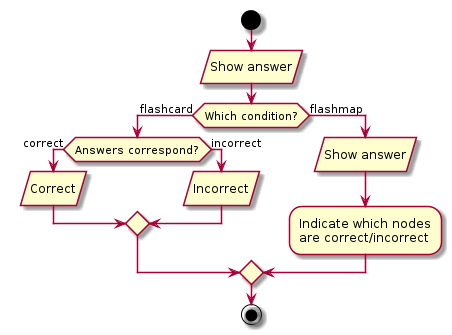
\includegraphics[width=.8\textwidth]{img/learningclient.png}
    \caption{An activity diagram displaying the prompting of an instance to the user}
    \label{fig:learningclient}
\end{figure}

\subsection{Read source}

\subsection{Flashcard prompt}

\subsection{Flashcard response}

\subsection{Flashmap prompt}

\subsection{Flashmap response}

\subsection{Finished learning}

\subsection{No more instances}

\section{Other views}

\subsection{Login screen}

\subsection{Test}

\subsection{Questionnaire}

\subsection{Debriefing}

\subsection{Main window}

\subsection{Help}

\subsection{Learning progress}
\label{sec:learningprogress}

